\documentclass[11pt]{article}

\usepackage[top=1in, bottom=1in, left=1in, right=1in]{geometry}
\usepackage{amsfonts}
\usepackage{graphicx}

\def\eq1{y=\displaystyle{\frac{x}{3x^2+x+1}}}
\def\sometext{Remember to label the axis}

\begin{document}

\title{Use Pacakges \LaTeX}
\author{Fan Cheng}
\date{\today}
\maketitle

The set of Natural numbers is denoted by $\mathbb{N}$. 

The set of integers is denoted by $\mathbb{Z}$. 

The set of real number is denoted by $\mathbb{R}$

Graph $\eq1$.

\sometext

\begin{center}
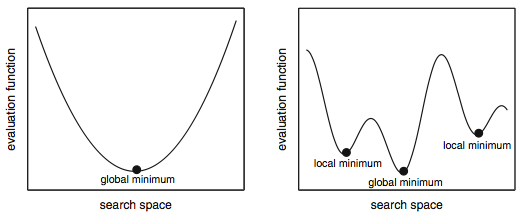
\includegraphics[width=5in, height=3in, angle=45]{a.png}
\end{center}

Note that when inserting pics, the pics should be put in the same folder containing the .tex file.

\end{document}
